% !TEX root = A0.MiTFG.tex

\chapter{Evaluación y resultados}

Este capítulo evalúa de forma comparativa la línea base y las dos etapas de mejora. La pregunta experimental no se limita a comprobar si Widevine reproduce, sino a determinar qué ocurre cuando una petición abandona el flujo legítimo, si la decisión queda asociada a una sesión y qué respuesta produce el sistema cuando el comportamiento se repite. Para evitar que la descripción de la implementación sustituya a la evidencia, los resultados se obtuvieron mediante una batería automatizada, reproducción real en navegador, capturas PCAP y exportaciones del estado de Redis.

La ejecución final comprendió 65 comprobaciones funcionales: 12 sobre Fase~0, 21 sobre Fase~1 y 32 sobre Fase~2. Todas produjeron el resultado esperado. La campaña temporal añadió 240 observaciones, con 20 repeticiones por combinación de fase y operación. Los datos originales se conservaron en \texttt{evidencias}, junto con scripts de repetición, capturas, logs, resúmenes HTTP sin tokens y huellas SHA-256.

\section{Escenarios de evaluación}

La evaluación siguió siempre el mismo orden. Primero se comprobó la disponibilidad del entorno y una reproducción legítima. Después se introdujeron credenciales o contextos incorrectos y, por último, se ejecutaron los escenarios con estado: concurrencia, detención de sesión, score y bans. Fase~1 se reinició antes de cada bloque que requería estado vacío; Fase~2 partió de Redis limpio. Esta separación impidió que una sesión anterior o un contador de riesgo contaminara el caso siguiente.

La Tabla~\ref{tab:escenarios-evaluacion} resume la matriz. El símbolo ``---'' indica que el concepto no existe en la fase correspondiente, no que la prueba se haya omitido accidentalmente.

\begin{table}[H]
\centering
\caption{Escenarios de la batería comparativa}
\label{tab:escenarios-evaluacion}
\begin{tabularx}{\textwidth}{Yp{0.19\textwidth}p{0.19\textwidth}p{0.19\textwidth}}
\toprule
\textbf{Escenario} & \textbf{Fase 0} & \textbf{Fase 1} & \textbf{Fase 2} \\
\midrule
Usuario autorizado & Reproducción permitida & Reproducción permitida & Reproducción permitida \\
Usuario sin \textit{entitlement} & Configuración 403 & Sesión 403 & Sesión 403 \\
Ruta \texttt{license/no\_auth} & Disponible & 401/404 & 401/404 \\
Origen y licencia internos & Puertos publicados & Sin publicación & Sin publicación \\
Token ausente o alterado & Solo controla ruta oficial & 401 & 401 \\
Activo o sesión distintos & Sin sesión de playback & 403/409 & 403/409 \\
Token después de detener & --- & 401 & 401 \\
Segunda reproducción & Sin límite & 409 & 409 y señal de riesgo \\
Abuso reiterado & Sin detección & Rechazo puntual & Score, eventos y ban \\
Recuperación administrativa & --- & --- & Retirada de ban \\
\bottomrule
\end{tabularx}
\end{table}

Se emplearon dos cuentas: una con acceso a \texttt{sintel-widevine} y otra sin activos permitidos. En las fases endurecidas cada login incluyó un \texttt{deviceId}; la sesión resultante se utilizó para manifest, heartbeat, contenido y licencia. Las pruebas negativas alteraron una sola condición cada vez: credencial, activo, identificador de sesión o estado de la reproducción.

La evidencia de red se adquirió dentro del espacio de red del contenedor CDN. En Fase~1 se conservaron 62 paquetes que contienen 17 solicitudes y 17 respuestas HTTP. En Fase~2 se generaron dos PCAP: 111 paquetes para concurrencia y 83 para fallos de autenticación. Su agregado PCAPNG contiene 194 paquetes. Los resúmenes JSON se generaron con TShark sin exportar \texttt{Authorization}; los PCAP brutos sí pueden contener tokens efímeros de laboratorio. Como en el Capítulo~4, no se intentó interpretar una licencia Widevine ni obtener claves desde la captura.

Durante la primera ejecución apareció una desviación relevante. Fase~2 no contrastaba la cabecera \texttt{X-Playback-Session-Id} en \texttt{/license}; una prueba con sesión distinta llegó al proxy interno y terminó en HTTP~500. La suite inicial obtuvo 64 de 65 casos. Se añadió la comprobación antes del reenvío y se repitió la batería completa: la misma solicitud pasó a devolver \texttt{409 SESSION\_MISMATCH} y el resultado final fue 65 de 65. La incidencia y ambas observaciones se conservan en \texttt{evidencias/resultados/incidencia\_binding\_licencia\_fase2.json}.

\section{Métricas utilizadas}

Se registraron métricas funcionales y operativas. Las primeras fueron el código HTTP, el motivo estructurado, la disponibilidad de caminos alternativos, la creación de eventos, el score y la presencia de bans. Las segundas fueron el tiempo de respuesta de endpoints locales y una instantánea del consumo de contenedores. Una reproducción se consideró válida solo cuando el navegador cargó el manifest, obtuvo licencias y mostró el vídeo en ejecución; no se aceptó únicamente el mensaje de la interfaz.

La duración HTTP se midió desde el inicio de la solicitud hasta la lectura completa de la respuesta. Se realizaron 20 repeticiones por operación. Este tamaño se eligió para mantener la prueba de Fase~1 dentro de su límite de 20 logins por minuto. En Fase~2 se limpió Redis antes de cada ciclo temporal: de otro modo, medir veinte heartbeats consecutivos habría activado deliberadamente la regla antifraude y habría mezclado rendimiento con respuesta de seguridad.

\subsection{Tiempo de respuesta}

La Tabla~\ref{tab:latencias-evaluacion} presenta mediana y percentil 95. En Fase~0, ``autorizar reproducción'' corresponde a \texttt{/playback/config}; en las fases restantes corresponde a crear \texttt{/playback/session}. Manifest, heartbeat y parada no tienen equivalente en la línea base porque Fase~0 no mantiene una sesión de reproducción diferenciada.

\begin{table}[H]
\centering
\caption{Tiempos de respuesta observados, 20 muestras por operación}
\label{tab:latencias-evaluacion}
\begin{tabularx}{\textwidth}{p{0.12\textwidth}Yp{0.18\textwidth}p{0.18\textwidth}}
\toprule
\textbf{Fase} & \textbf{Operación} & \textbf{Mediana (ms)} & \textbf{P95 (ms)} \\
\midrule
0 & Login & 15,100 & 17,779 \\
0 & Autorizar reproducción & 15,639 & 24,857 \\
\midrule
1 & Login & 15,489 & 26,231 \\
1 & Autorizar reproducción & 15,072 & 24,332 \\
1 & Manifest & 44,166 & 79,107 \\
1 & Heartbeat & 9,347 & 20,541 \\
1 & Detener sesión & 15,639 & 27,150 \\
\midrule
2 & Login & 18,659 & 32,617 \\
2 & Autorizar reproducción & 11,293 & 31,528 \\
2 & Manifest & 84,614 & 125,130 \\
2 & Heartbeat & 19,595 & 32,182 \\
2 & Detener sesión & 29,335 & 32,360 \\
\bottomrule
\end{tabularx}
\end{table}

El login de Fase~1 mantuvo una mediana prácticamente igual a Fase~0. Fase~2 elevó esa mediana un 20,5\% respecto a Fase~1. El heartbeat pasó de 9,347 a 19,595~ms y la parada, de 15,639 a 29,335~ms. Estas diferencias son coherentes con el acceso adicional a Redis y la creación de eventos, pero no constituyen un benchmark de producción: se midieron en un único equipo y con tráfico secuencial.

El manifest presentó mayor variabilidad. Fase~2 obtuvo una mediana de 84,614~ms frente a 44,166~ms en Fase~1. Ambas rutas descargan el MPD desde la infraestructura pública de Shaka antes de responder, por lo que la cifra combina red externa, reescritura local, planificación de Docker y, en Fase~2, persistencia y observabilidad. En consecuencia, no es correcto atribuir toda la diferencia a Redis.

\subsection{Número de accesos bloqueados}

Se contabilizaron únicamente respuestas 4xx esperadas; un error 5xx se consideraría fallo de la prueba. Fase~0 produjo tres rechazos válidos en su camino oficial: credenciales incorrectas, usuario sin permiso y licencia oficial sin token. Sin embargo, mantuvo accesibles el origen y la ruta alternativa de licencia. El PCAP del bypass conserva dos \texttt{POST /license/no\_auth} con HTTP~200 sin login ni configuración previa.

Fase~1 produjo 14 rechazos esperados y Fase~2, 17. La cifra mayor no significa por sí sola que Fase~2 sea ``un 21\% más segura'', pues contiene tres escenarios adicionales. Su significado es funcional: todas las variantes negativas de las fases endurecidas terminaron en 401, 403, 404 o 409, sin errores 5xx en la regresión final de esas dos fases. Entre ellas se encuentran token alterado, activo distinto, sesión distinta, contenido no asociado, ruta heredada y token posterior a la parada.

\subsection{Detección de abuso}

El rechazo de concurrencia permite distinguir prevención de detección. Fase~1 devolvió 409 ante una segunda sesión, pero no conservó una puntuación. En Fase~2 se mantuvo una sesión válida y se enviaron cinco solicitudes adicionales. Las cinco devolvieron \texttt{CONCURRENCY\_LIMIT}; el score observado después de cada una fue 0, 25, 50, 75 y 100. El primer rechazo únicamente inició el contador y los cuatro siguientes añadieron 25 puntos. Al llegar a 100 se creó un ban de cuenta de 30 minutos con razón \texttt{AUTO\_BAN:REPEATED\_CONCURRENCY\_VIOLATION}.

La exportación Redis conserva cinco eventos \texttt{playback.concurrency\_rejected}, cuatro \texttt{risk.incremented}, un \texttt{ban.created}, un \texttt{ban.cleared} y la parada final. Mientras el ban estuvo activo, el manifest respondió 401. La Figura~\ref{fig:fase2-laboratorio-bloqueo}, incluida en el capítulo anterior, muestra este estado; el PCAP registra seis \texttt{POST /playback/session}: una creación 201 y cinco conflictos 409.

El segundo escenario envió ocho contraseñas incorrectas desde el mismo dispositivo. Todas recibieron 401, se creó \texttt{AUTH\_FAILURE\_BURST} durante 15 minutos y el manifest posterior quedó rechazado. Al tratarse de una respuesta directa sobre dispositivo, el score de cuenta permaneció en cero. La Figura~\ref{fig:evaluacion-ban-dispositivo} muestra el resultado visible y la secuencia registrada.

\begin{figure}[htbp]
    \centering
    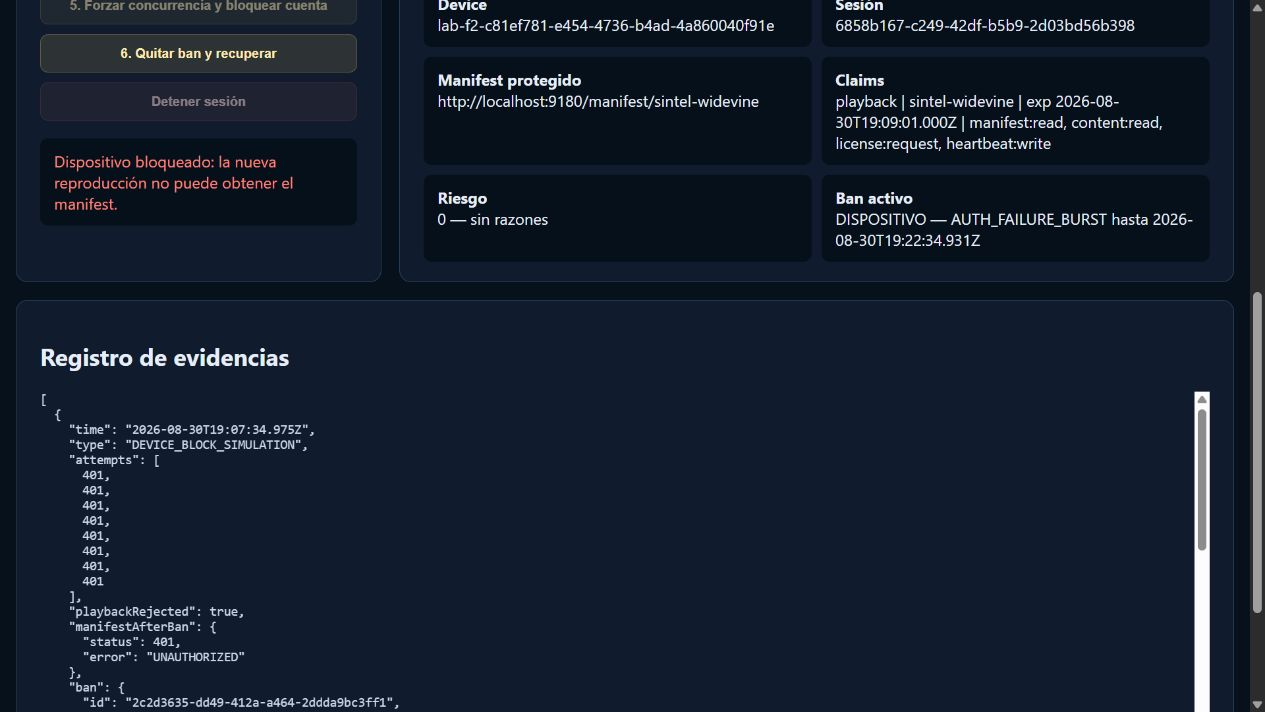
\includegraphics[width=0.98\textwidth]{figuras/evaluacion-fase2-ban-dispositivo.png}
    \caption{Evaluación de Fase~2 tras ocho fallos de autenticación y activación del ban de dispositivo.}
    \label{fig:evaluacion-ban-dispositivo}
\end{figure}

En ambos escenarios el plano administrativo permaneció operativo, retiró el ban y permitió renovar la credencial o crear una sesión nueva si la anterior había expirado. El score de cuenta no se reinició al retirar el ban de concurrencia; permaneció en 100 como evidencia del comportamiento previo.

\subsection{Impacto en rendimiento}

La instantánea de contenedores mostró 30,39~MiB para el plano de control de Fase~1 y 38,52~MiB para el de Fase~2. Redis utilizó 5,13~MiB adicionales. Los dos contenedores Varnish se mantuvieron alrededor de 96~MiB. El uso puntual de CPU fue inferior al 1\% en los componentes citados. Estos valores describen el laboratorio en reposo después de la campaña; no deben interpretarse como capacidad máxima ni como prueba de carga.

El coste funcional fue reducido en términos absolutos: ninguna mediana local superó 30~ms salvo la obtención del manifest, condicionada por el upstream externo. Fase~2 sí mostró más latencia en login, heartbeat y parada, además de aproximadamente 13,3~MiB sobre la suma del plano de control y Redis frente al plano de control de Fase~1. A cambio, incorpora estado compartido, eventos, score y respuesta administrativa, capacidades ausentes en las fases anteriores.

\section{Evaluación del sistema base}

Fase~0 superó sus comprobaciones legítimas. El usuario permitido reprodujo Widevine y el activo CENC local; el usuario sin \textit{entitlement} recibió 403 al solicitar configuración. La ruta oficial de licencia devolvió 401 sin token. Por tanto, la línea base no es un sistema sin controles, sino un sistema cuyos controles no cubren todos los caminos equivalentes.

La diferencia apareció al abandonar el cliente oficial. El origen respondió HTTP~200 en \texttt{localhost:8081} y el servidor de licencias publicó su health en \texttt{localhost:8082}. Una solicitud binaria artificial a \texttt{/license/no\_auth} alcanzó la lógica de proxy sin recibir 401, 403 o 404; el challenge inválido terminó en 500 y la respuesta conservó \texttt{X-Phase0-Weakness}. Más importante, el PCAP de reproducción real ya analizado en el Capítulo~4 contiene una preflight y dos \texttt{POST /license/no\_auth} con respuesta 200, sin login ni \texttt{/playback/config}. Esta combinación evita confundir ``ruta alcanzable'' con ``challenge Widevine válido''.

La demostración ClearKey confirmó también que el MPD, las inicializaciones y los primeros segmentos podían recuperarse sin URI de licencia cuando la clave de laboratorio era conocida. Este resultado no rompe Widevine; muestra que cifrar el activo no compensa la exposición simultánea del contenido y del material necesario para descifrar otro activo CENC controlado.

En conjunto, Fase~0 bloqueó el uso no permitido dentro de la interfaz oficial, pero no gobernó de extremo a extremo el acceso al origen y al proxy de licencia. Tampoco pudo revocar una reproducción concreta, limitar concurrencia ni correlacionar eventos por sesión.

\section{Evaluación del sistema propuesto}

Fase~1 mantuvo la reproducción Widevine real y eliminó los caminos alternativos. El PCAP de evaluación contiene login, creación de sesión, manifest, dos solicitudes de licencia y parada. Los cuatro casos negativos del laboratorio produjeron 401, 401, 409 y 403, como recoge la Figura~\ref{fig:evaluacion-fase1-negativas}. La distribución completa del PCAP fue de seis respuestas 200, una 201, seis preflight 204, dos 401, una 403 y una 409.

\begin{figure}[htbp]
    \centering
    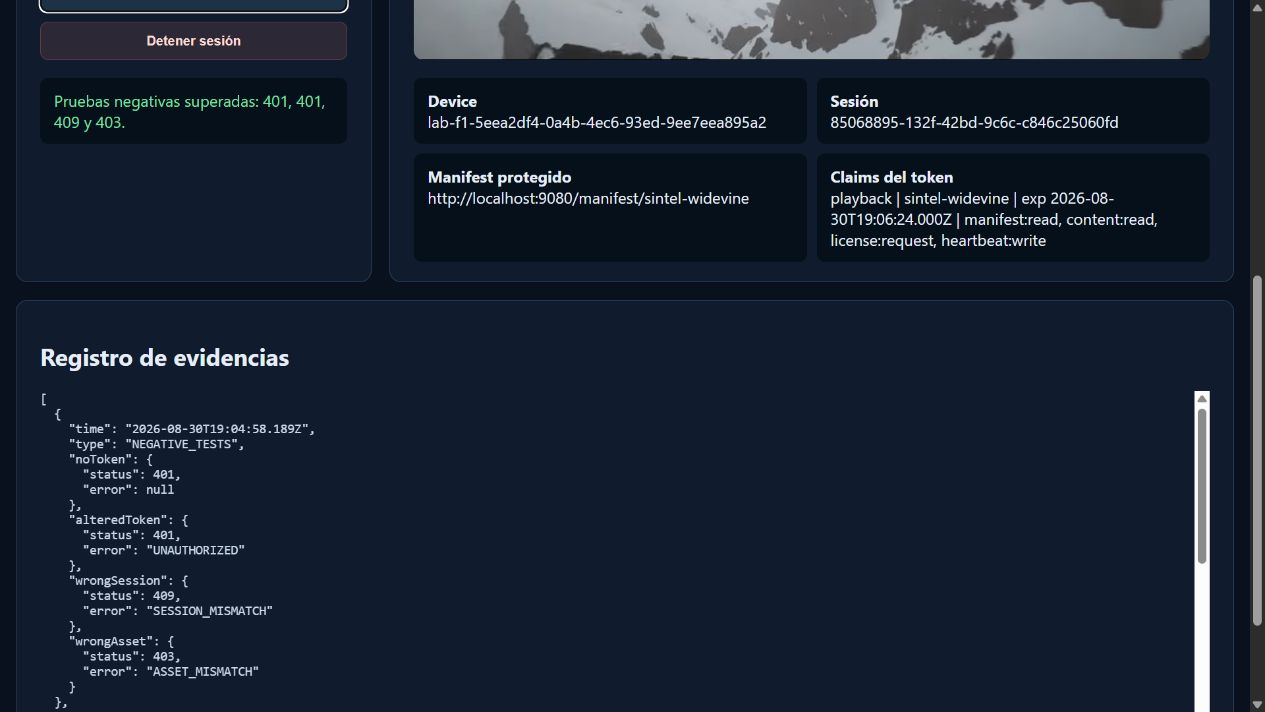
\includegraphics[width=0.98\textwidth]{figuras/evaluacion-fase1-pruebas-negativas.png}
    \caption{Pruebas negativas de Fase~1 con reproducción legítima activa y binding de token, activo y sesión.}
    \label{fig:evaluacion-fase1-negativas}
\end{figure}

La topología confirmó que origen, servidor de licencias y plano de control no tienen bindings en el anfitrión. \texttt{/license/no\_auth} devolvió 401 sin credencial y 404 con un token válido, lo que demuestra que la ruta no se limita a ocultarse tras autenticación: ha desaparecido del backend. Después de detener la sesión, el mismo token de reproducción devolvió 401 al solicitar el manifest.

Fase~2 conservó estos 14 comportamientos preventivos y añadió administración, detección y recuperación. La cuenta sin \textit{entitlement} tampoco pudo consultar \texttt{/admin/overview}. Los dos escenarios de abuso generaron los bans esperados y el plano administrativo los retiró sin perder observabilidad. El PCAP de concurrencia registró 35 solicitudes y respuestas HTTP; el de autenticación, 25. Los estados JSON contienen, respectivamente, 19 y 18 eventos de servidor.

La corrección de \texttt{/license} durante la campaña refuerza una conclusión metodológica: compartir arquitectura no garantiza que dos fases apliquen exactamente las mismas validaciones. La regresión automatizada descubrió una diferencia que no era visible en la reproducción legítima. Tras la corrección, manifest, contenido y licencia contrastan de forma coherente la sesión indicada por el cliente.

\section{Comparativa de resultados}

La Tabla~\ref{tab:comparativa-final} concentra el resultado final. ``Rechazo'' significa respuesta preventiva; ``detección'' exige además conservar una señal, y ``respuesta'' implica modificar el estado de acceso. Esta distinción evita atribuir a Fase~1 una capacidad antifraude que no implementa.

\begin{table}[H]
\centering
\caption{Comparación final de las tres fases}
\label{tab:comparativa-final}
\begin{tabularx}{\textwidth}{Yp{0.18\textwidth}p{0.18\textwidth}p{0.18\textwidth}}
\toprule
\textbf{Propiedad} & \textbf{Fase 0} & \textbf{Fase 1} & \textbf{Fase 2} \\
\midrule
Widevine legítimo & Funciona & Funciona & Funciona \\
Ruta pública de licencia & Sí & No & No \\
Origen/licencia publicados & Sí & No & No \\
Token efímero de playback & No & Sí, 90~s & Sí, 90~s \\
Binding cuenta--dispositivo--activo--sesión & No & Sí & Sí \\
Revocación por parada & No & Sí & Sí \\
Concurrencia & Sin control & Rechazo 409 & 409 y score \\
Eventos persistentes & No & No & Sí, Redis \\
Ban automático & No & No & Cuenta y dispositivo \\
Recuperación administrativa & No & No & Sí \\
Comprobaciones finales & 12/12 & 21/21 & 32/32 \\
\bottomrule
\end{tabularx}
\end{table}

La mejora principal de Fase~1 fue cualitativa: el acceso dejó de depender de que el usuario utilizara la interfaz prevista. El mismo control se aplicó en manifest, contenido y licencia, y los servicios internos dejaron de estar publicados. Fase~2 no volvió ``más cifrado'' el contenido; añadió memoria y capacidad de reacción sobre una ruta ya autorizada.

Los tiempos muestran que esa memoria tiene coste, aunque permanece pequeño en el laboratorio. No se observó una penalización uniforme: la mediana de creación de sesión de Fase~2 fue incluso menor que la de Fase~1, mientras que heartbeat y parada aproximadamente se duplicaron. Esta dispersión, junto con los percentiles 95, aconseja no convertir una campaña secuencial de 20 muestras en una afirmación de escalabilidad.

\section{Discusión técnica}

\subsection{Mejoras observadas}

La primera mejora es la eliminación del bypass. En la línea base, una decisión correcta de \textit{entitlement} coexistía con un proxy que no recibía identidad. En las fases endurecidas no existe un camino equivalente: el frontal y el backend exigen una credencial de reproducción y el servidor interno de licencias solo acepta contexto procedente del plano de control.

La segunda es la reducción de la ventana de reutilización. El token de reproducción expira en 90 segundos, se liga a una sesión y se renueva mediante heartbeat. Detener la sesión invalida su uso aunque el token todavía sea criptográficamente válido. Activo, cuenta, dispositivo y sesión se contrastan antes de servir recursos sensibles.

La tercera mejora es observable únicamente en Fase~2. Los rechazos repetidos dejan de ser respuestas independientes y forman una señal acumulada. Los eventos Redis permitieron reconstruir la secuencia desde el login hasta \texttt{ban.created}, el rechazo posterior, \texttt{ban.cleared} y \texttt{playback.stopped}. Esta trazabilidad es la base para operación y análisis posterior.

\subsection{Limitaciones persistentes}

El laboratorio utiliza HTTP y secretos de demostración incluidos en Docker Compose. Un despliegue real necesitaría TLS extremo a extremo, rotación y custodia externa de claves. El formato de token firmado empleado por el prototipo tiene dos segmentos y no constituye un JWT RFC~7519 completo, tal como se explicó en el capítulo de implementación.

El activo Widevine, su MPD y el servicio CWIP pertenecen a infraestructura pública de pruebas. Los segmentos Widevine no atraviesan el origen privado del laboratorio. Por ello, la campaña demuestra gobierno local del manifest y la licencia, pero no cuantifica una CDN comercial ni una política de licencia de producción.

Los umbrales de Fase~2 son ilustrativos. No se han calibrado con una población real, falsos positivos conocidos, diversidad geográfica o dispositivos heterogéneos. Redis funciona sin persistencia, replicación ni alta disponibilidad para facilitar el reinicio. Las medidas temporales proceden de un solo equipo, tráfico secuencial y 20 muestras; sirven para comparar este prototipo, no para dimensionar producción.

El \texttt{deviceId} lo genera JavaScript y no constituye una prueba fuerte de identidad de hardware. El watermark es visible, pero no forense. Tampoco se evalúan HDCP, robustez del CDM, seguridad del sistema operativo, captura de pantalla ni compromiso del dispositivo final.

\subsection{Ataques que seguirían siendo posibles}

Un atacante que obtuviera un token de reproducción válido y pudiera reproducir el mismo contexto de sesión y dispositivo dispondría de una ventana corta hasta la expiración o revocación. Al tratarse de una credencial bearer y de un identificador de dispositivo declarado por el cliente, el binding reduce reutilización accidental, pero no equivale a atestación criptográfica.

Un patrón distribuido y lento podría mantenerse por debajo de los umbrales o repartir actividad entre múltiples cuentas y dispositivos. Del mismo modo, compartir una cuenta de forma serial, sin sesiones simultáneas, no activa el control de concurrencia. Un adversario también podría dirigir denegación de servicio contra Varnish, el plano de control o Redis, ámbitos no cubiertos por esta campaña funcional.

Finalmente, ningún control de acceso impide por sí solo que un usuario autorizado grabe la salida ya descifrada. DRM, tokens y bans gobiernan la obtención de licencia y recursos; no eliminan el denominado \textit{analog hole}. La marca visible aporta atribución limitada, pero puede recortarse o taparse.

\subsection{Mitigaciones posibles}

La evolución natural sería reemplazar los secretos locales por un gestor de claves, emplear TLS externo y mTLS entre servicios, y utilizar un proveedor de identidad con tokens estándar, rotación de claves y revocación. El identificador de dispositivo podría reforzarse con atestación, claves no exportables o señales del SDK DRM, siempre evaluando privacidad y compatibilidad.

En la distribución convendría incorporar URLs o cookies firmadas de CDN, autorización también sobre segmentos, políticas Widevine de producción y rotación de claves por activo o periodo. Un watermark forense individualizado complementaría al visible cuando el riesgo justifique su coste.

Para detección, los eventos deberían enviarse a una plataforma externa con retención, correlación entre regiones y control de acceso. Los umbrales se calibrarían con tráfico histórico, cohortes y métricas de falsos positivos. Rate limiting distribuido, protección WAF/DDoS y Redis persistente y replicado completarían la disponibilidad. Estas medidas no alteran la conclusión experimental: la defensa efectiva procede de combinar DRM con autorización extremo a extremo, contexto de sesión, observabilidad y respuesta, no de confiar en una única capa.
